%% Information-consistent evaluation of battery RUL (methods paper)
\documentclass[preprint,12pt]{elsarticle}

\usepackage{amsmath,amssymb}
\usepackage{array}
\usepackage{booktabs}
\usepackage{graphicx}
\usepackage{hyperref}
\usepackage{siunitx}
\usepackage{microtype}
\usepackage{xurl}
\usepackage{setspace}
\setstretch{1.15}
\setlength{\emergencystretch}{2em}
\renewcommand{\topfraction}{0.9}
\renewcommand{\bottomfraction}{0.8}
\renewcommand{\textfraction}{0.07}
\renewcommand{\floatpagefraction}{0.85}

\graphicspath{{figures/}{../ei_manuscript/figures/pub/}}
\makeatletter
\def\ps@pprintTitle{%
  \let\@oddhead\@empty
  \let\@evenhead\@empty
  \def\@oddfoot{\hfill\footnotesize\itshape\today}%
  \let\@evenfoot\@oddfoot}
\makeatother

\begin{document}

\begin{frontmatter}

\title{Information-Consistent Evaluation of Li-ion Battery Remaining Useful Life:
An Information-Level Framework for Retrospective Oracles}

\author[1]{Jiapei Jiang\corref{cor1}}
\ead{jjp@mails.guet.edu.cn}
\cortext[cor1]{Corresponding author.}
\address[1]{School of Business, Guilin University of Electronic Technology, Guilin 541004, China}

\begin{abstract}
Data-driven remaining useful life (RUL) prediction for lithium-ion batteries typically ranks models by test error while omitting the information boundary at prediction time.
A common leakage arises when the relative-cycle feature $\mathrm{cycle\_norm}=t/T$ and the label $\mathrm{RUL}_t=T-t$ share the same target lifetime~$T$.
Because~$T$ is unknown online, that feature is a retrospective oracle and is not legitimate for deployment claims.
We propose an \emph{information-consistent} evaluation protocol with four elements: a nested information hierarchy (L0: raw~$t$; L1: leave-target population prior $t/T^{\mathrm{prior}}$; L1P: SOH-matched sibling local prior; L2: target oracle $t/T_{\mathrm{target}}$), declared fit protocols (within-cell retrospective Protocol~A; strict leave-target Protocol~B), feature-source auditing, and a structured report standard.
End-of-life is the first cycle with SOH$\le 0.7$; cells that never reach the threshold are right-censored.
MLP and Patch-TF are matched ranking instruments only.
On Severson Protocol~B ($n{=}24$), median MLP RUL RMSE falls from $222.1$ at L0 to $12.0$ at L2 (Wilcoxon $p=1.2{\times}10^{-7}$), showing that the information level dominates ranking.
Counter-intuitively, under NASA Protocol~A the local prior L1P beats the target oracle L2 (B0005: $5.06$ vs.\ $23.58$).
The mechanism is learnability, not ``less information is better'': the L2 clock in the test window lies outside its training support, so the network overestimates late-life RUL, whereas L1P stays inside a proximate SOH match and avoids temporal extrapolation.
The inversion reverses under Protocol~B (L1P $30.3$ vs.\ L2 $12.0$).
The contribution is an auditable, reproducible RUL benchmarking standard---not a new predictive architecture.
\end{abstract}

\begin{keyword}
Lithium-ion battery \sep RUL \sep Information availability \sep Evaluation protocol \sep Retrospective oracle \sep Leave-one-cell-out
\end{keyword}

\end{frontmatter}

\section{Introduction}
\label{sec:intro}

Data-driven remaining useful life (RUL) prediction is central to battery management systems (BMS)~\cite{hu2019rser,xiong2018soh}.
Deep sequence models---Transformers, Mamba, physics-informed nets, and related hybrids---continue to reset reported accuracy under fixed feature sets~\cite{lipu2018,wang2024gce,xu2025meas,yang2025batteries,zhang2025batlinet,deng2025piml,huang2025rulmamba,sun2026sgdits}.
Leaderboard-style comparisons, however, often leave a more basic question unanswered: at prediction cycle~$t$, which information is the model allowed to use?

A widespread but under-audited leakage arises in the construction of relative-life features.
Researchers commonly encode cycle progress as
\begin{equation}
\mathrm{cycle\_norm}=\frac{t}{T},
\end{equation}
with label $\mathrm{RUL}_t=T-t$, where~$T$ is the cell's end-of-life (EOL).
Because the same~$T$ that defines the label also enters $X_t$, the learner answers a retrospective question.
Removing the channel or fixing the time scale collapses many reported gains.
Geslin et al.\ require lifetime features to match the intended use case~\cite{geslin2023joule}; recent LOCO and group-wise studies show that same-cell random splits and blurred information boundaries inflate apparent accuracy~\cite{ali2026loco,barua2026predictor,madani2025groupkfold}.
On NASA B0005, when record length was used as~$T$, Patch-TF RUL RMSE rose from $2.28\pm0.96$ with this channel to $18.83\pm3.88$ without it~\cite{saha2007nasa}.

Although leakage is well studied in machine learning~\cite{kaufman2012leakage,kapoor2023leakage}, three evaluation gaps remain specific to battery RUL:
\begin{enumerate}
\item \textbf{No operable nested information hierarchy.}
Few studies state how far the EOL constant~$T$ may enter $X_t$, or handle intermediate collapse (e.g., when a population prior coincides with the target oracle on lifetime-homogeneous data).
\item \textbf{Information level conflated with fit protocol.}
Within-cell retrospective splits are often reported alongside leave-target generalisation without separating label construction from input legitimacy.
\item \textbf{Irreproducible baselines and missing report fields.}
``Persistence'' is rarely named, and structured fields for information level, scaler provenance, and channel support status are almost never required beside the RMSE table.
\end{enumerate}

This paper therefore addresses a protocol boundary, not an architecture race: how do error and ranking change with the prediction-time information set $\mathcal{I}_t$?
We write
\begin{equation}
\boxed{\operatorname{Rank}(M_1,\ldots,M_k\mid \mathcal{I}_t)\;=\;f(\mathcal{I}_t)}
\end{equation}
and answer with four cycle channels---L0 (raw~$t$), L1 (leave-target population prior $t/T^{\mathrm{prior}}$), L1P (SOH-matched sibling local prior), and L2 (target oracle $t/T_{\mathrm{target}}$)---together with fit Protocols~A (within-cell retrospective) and~B (strict leave-target), named Persistence baselines, first-EOL labelling, and right-censoring.
MLP and Patch-TF are matched ranking instruments only.

Two findings expose the fragility of current ranking practice and a learnability limit of the learner.
First, under Severson Protocol~B ($n{=}24$), median MLP RUL RMSE falls from $222.1$ at L0 to $12.0$ at L2 (Wilcoxon $p=1.2{\times}10^{-7}$): target-life information dominates ranking.
Second, under NASA Protocol~A, the weaker local prior L1P can beat the full-target oracle L2 (B0005: $5.06$ vs.\ $23.58$).
Error decomposition shows why: after a chronological split, every scored L2 test window lies out of training support, so the network compresses late-life variation and systematically over-predicts RUL; L1P interpolates inside an SOH neighbourhood and avoids that extrapolation.
Sufficient information that is not learnable on the scored windows does not become a predictive advantage; under Protocol~B the ordering reverses (L1P $30.3$ vs.\ L2 $12.0$).

\paragraph{Contributions.}
(C1)~\textbf{Core protocol.}
L0/L1/L1P/L2 information levels, first-EOL definition with right-censoring, separated Protocols~A/B, and a per-input provenance audit that records channel support status.
(C2)~\textbf{Mechanism.}
Boundary conditions for ``local prior beats target oracle'' (out-of-support clock; SOH-neighbourhood coverage) and evidence that the inversion reverses under Protocol~B and on CALCE.
(C3)~\textbf{Reporting standard.}
A one-row modular report template that makes the information condition a mandatory audit field, usable as an evaluation shell for platforms such as BatteryML~\cite{zhang2024batteryml}.
The contribution is methodology for auditable RUL benchmarking, not a new network.

\section{Related work}
\label{sec:related}

\paragraph{Leakage as illegitimate target information.}
Kaufman et al.\ define leakage as target information that should not be legitimately available to the learner~\cite{kaufman2012leakage}.
Kapoor and Narayanan show that such leakage produces irreproducible machine-learning leaderboards~\cite{kapoor2023leakage}.
Similar inflation appears when row-wise splits leak subject identity~\cite{rosenblatt2024}.
In batteries, random within-cell splits and optimistic validation can likewise overstate SOH/RUL accuracy relative to cell-held-out tests~\cite{barua2026predictor,ali2026loco}.
RUL labels \emph{must} use a future EOL by definition; the illegitimate step under an online claim is copying that future into $X_t$.

\paragraph{BMS monitoring, SOH, and RUL.}
On-board monitoring and state estimation remain core BMS requirements~\cite{hu2019rser}.
SOH reviews separate electrochemical diagnosis from data-driven mapping~\cite{xiong2018soh}.
RUL surveys catalogue filters, neural nets, and hybrid learners~\cite{lipu2018,wang2024gce,xu2025meas,yang2025batteries}, but they often leave the cycle clock outside the evaluation protocol.
Capacity regeneration and mixed degradation modes further break a constant-fade story~\cite{birkl2017,aliakbari2025fusedr,fan2026meas}.

\paragraph{Data-driven RUL learners and recent benchmarks.}
Classical prognostic baselines remain useful reference points~\cite{saha2009compare}.
Recent work spans inter-cell deep learning~\cite{zhang2025batlinet}, physics-informed early-life predictors~\cite{deng2025piml,oyewole2025uq}, and sequence models such as Transformers, Mamba, and dual-path state-space networks~\cite{vaswani2017,nie2023patchtst,huang2025rulmamba,li2026dpmamba,sun2026sgdits,yi2025jps,tian2025energy,ge2025koopman,li2025adapt,wang2025jes}.
Open platforms and multi-dataset benchmarks show that architecture tables alone do not fix evaluation regimes~\cite{zhang2024batteryml,tan2025batterylife,li2024lifetime}.
MC-Dropout is retained here only as an appendix UQ foil~\cite{gal2016}.
We use a matched Patch-TF versus MLP pair only as a ranking instrument under controlled $\mathcal{I}_t$, not as an architecture claim.

\paragraph{What benchmark platforms do and do not audit.}
BatteryML standardises data ingestion, feature extraction, and model training for degradation studies~\cite{zhang2024batteryml}; BatteryLife aggregates 16 corpora and benchmarks 18 methods under a common pipeline~\cite{tan2025batterylife}.
These platforms make data and model choices reproducible, which is complementary to the present work.
To our knowledge, however, neither makes the prediction-time information level a required evaluation field: the scaler source, the $T$ definition, the within-cell versus leave-target protocol, and the presence of $t/T_{\mathrm{target}}$ are not reported as separate auditable rows.
We do not claim that either platform is leaky; we claim that their reporting cards leave the information condition implicit, so a model that consumes $T_{\mathrm{target}}$ and a model that does not can appear in the same table without distinction.
The ladder proposed here can be recorded alongside their dataset and model cards as an additional field.

\paragraph{Lifetime datasets, features, and evaluation protocols.}
Public cycle-life corpora include NASA PCoE~\cite{saha2007nasa,saha2009compare}, CALCE~\cite{he2011calce}, and the MIT/Stanford set~\cite{severson2019nature}; expanded lifelong and multi-condition datasets continue to appear~\cite{li2024lifetime,tan2025batterylife,zhang2025batlinet}.
Geslin et al.\ showed that feature legitimacy depends on the use case~\cite{geslin2023joule}.
Field data add further availability constraints~\cite{sulzer2021joule}.
Cell-grouped and LOCO validation are increasingly recommended when the claim is out-of-cell generalization~\cite{roman2021,madani2025groupkfold,ali2026loco,barua2026predictor}.
Our L2 channel $t/T_{\mathrm{target}}$ is a deliberate retrospective relative-life clock: informative for completed-life studies, but information-inconsistent under an online-valid claim.
The gap addressed here is an operational L0/L1/L1P/L2 ladder, named fit protocols, a support check for the cycle channel, and a fillable report row.

\section{Information-consistent protocol}
\label{sec:protocol}

\subsection{Observation set and lifetime}
\label{sec:Ot}

Prediction is cycle-level after completed discharge~$t$.
Capacity $Q_t$ is obtained by integrating discharge current.
SOH is $Q_t/Q_1$ on that cell.
EOL threshold is 0.7 throughout.
We define
\begin{equation}
T \;=\;
\begin{cases}
\min\{ \tau: \mathrm{SOH}_\tau \le 0.7\}, & \text{if the set is non-empty},\\
T_{\mathrm{record}}, & \text{otherwise (right-censored)},
\end{cases}
\end{equation}
and
\begin{equation}
\label{eq:rul}
\mathrm{RUL}_t \;=\; \max(0,\, T-t).
\end{equation}
Capacity regeneration after the first crossing does not reopen a positive countdown to a later crossing: $T$ and~\eqref{eq:rul} use one global first EOL.
Using the last recorded cycle instead of $T$ makes NASA B0005--B0007 look like identical lifetimes (record length 168) even though EOL values are 161, 106, and 167 (Table~\ref{tab:life}).

A cell that never crosses the threshold has a \emph{censored} lifetime: $T$ is then the end of observation, and $\mathrm{RUL}_t$ counts down to the record horizon rather than to a failure event.
We flag this case explicitly (Table~\ref{tab:life}) because absolute RUL errors on a censored cell are not comparable with errors on a cell that truly failed, even though all information levels share the same labels and their \emph{ranking} remains internally valid.
B0007 is the only censored cell in this study (final SOH $\approx 0.76$); its role is discussed in Section~\ref{sec:b0007}.

The observation set $\mathcal{O}_t$ may include
$\{Q_\tau,\overline{V}_\tau,\overline{I}_\tau,\overline{T}_\tau,\mathrm{std}(V)_\tau\}_{\tau\le t}$
(NASA; CALCE uses SOH and $t$ only),
the raw index~$t$,
and scalers fit on training time of the same cell (or leave-target siblings) only.
It excludes $T_{\mathrm{target}}$, $t/T_{\mathrm{target}}$, and any transform that needs the full target trajectory, except under the named L2 deliberate-oracle condition below.

Hard rule for online-valid inputs:
\begin{equation}
\boxed{T\in Y,\qquad T\notin X_t,\qquad X_t\subseteq\mathcal{O}_t.}
\end{equation}
L2 deliberately violates $T\notin X_t$; that violation is the oracle condition being measured, not an unnamed protocol error.

\subsection{Levels L0 / L1 / L2 and diagnostic L1P}
\label{sec:levels}

Only the cycle channel~$c_t$ changes; other input channels stay fixed.
Nesting is on the \emph{permitted lifetime constants} used to build~$c_t$, not on a claim that prediction-time observables about the target trajectory form a strict information filtration:
\begin{equation}
\label{eq:nested}
\begin{aligned}
\mathcal{K}_0&=\emptyset,&
\mathcal{K}_1&=\{T^{\mathrm{prior}}\},&
\mathcal{K}_2&=\{T^{\mathrm{prior}},T_{\mathrm{target}}\},\\
&\mathcal{K}_0\subset\mathcal{K}_1\subset\mathcal{K}_2,\\
c_t^{(0)}&=t,&
c_t^{(1)}&=\frac{t}{T^{\mathrm{prior}}},&
c_t^{(2)}&=\frac{t}{T_{\mathrm{target}}}.
\end{aligned}
\end{equation}
We write $\mathcal{I}_k$ for the evaluation condition that uses channel~$c_t^{(k)}$.
Here $T^{\mathrm{prior}}=\mathrm{median}\{T_i:i\in D_{\mathrm{train}}\}$ uses leave-target training cells only; $\mathrm{median}(T_{\mathrm{all}})$ is forbidden.
L2 is a \emph{deliberate oracle}: completed target life enters~$X_t$ by construction.
Relative to an online-valid claim ($T_{\mathrm{target}}$ unavailable at~$t$), the same channel is information-inconsistent; that online reading is stated only when the use case is online BMS.
Because $T^{\mathrm{prior}}$ and $T_{\mathrm{target}}$ are constants with respect to~$t$,
\begin{equation}
\label{eq:affine}
c_t^{(1)}=\alpha\,c_t^{(0)},\qquad
c_t^{(2)}=\beta\,c_t^{(0)},\qquad
\alpha=(T^{\mathrm{prior}})^{-1},\ \beta=T_{\mathrm{target}}^{-1},
\end{equation}
so L0/L1/L2 are mutually affine (strictly monotone) transforms of the same index~$t$ at the \emph{input} level.

\paragraph{What the affine identity does and does not imply.}
Equation~\eqref{eq:affine} is a statement about inputs, not about trained predictors.
Table~\ref{tab:affine} separates the three levels of the argument.
The identity guarantees the same ordering of cycles and the same information in an idealised function class; it does not guarantee equal network outputs, equal test error, or equal learnability.
Empirically, L1 and L2 predictions under Protocol~A differ by $0.02$--$0.25$ cycles on average ($\rho>0.97$), which is consistent with numerical scale robustness of the fitted network, whereas under Protocol~B their median RMSE differs by a factor of $2.8$.
The reconciliation is that an affine rescaling changes the numerical range on which the network is fitted, and therefore changes how it extrapolates outside that range; it does not change what the channel contains.
Section~\ref{sec:mechanism} uses this distinction to explain the L1P inversion.

\begin{table}[htbp]
\centering
\footnotesize
\caption{Affine identity versus empirical error equality. The table records what Equation~\eqref{eq:affine} proves, what it does not, and the observation that separates the two.}
\label{tab:affine}
\setlength{\tabcolsep}{4pt}
\begin{tabular}{@{}>{\raggedright\arraybackslash}p{0.28\linewidth}>{\raggedright\arraybackslash}p{0.17\linewidth}>{\raggedright\arraybackslash}p{0.47\linewidth}@{}}
\toprule
Statement & Status & Evidence / remark \\
\midrule
$c^{(1)}=\alpha c^{(0)}$, $c^{(2)}=\beta c^{(0)}$ with $\alpha,\beta>0$ & proved & Equation~\eqref{eq:affine}; strictly monotone in $t$ \\
L0/L1/L2 preserve the ordering of cycles & implied & monotone transform of the same index \\
Trained outputs satisfy $\hat y^{(1)}=\hat y^{(2)}$ & not implied & mean $|\hat y^{L1}-\hat y^{L2}|=0.02$--$0.25$ cycles under A ($\rho>0.97$); L1 $33.5$ vs.\ L2 $12.0$ under B \\
RUL RMSE invariant to rescaling & not implied & A: $23.62$ vs.\ $23.58$; clock $t/1000$: $23.11$; raw $t$: $14.92$ (B0005) \\
L1P is affine in $t$ & false by construction & SOH-indexed lookup, Eq.~\eqref{eq:l1p}; $\rho(\mathrm{L1P},\mathrm{L2})$ from $-0.12$ to $-0.82$ \\
\bottomrule
\end{tabular}
\end{table}

\paragraph{Training support.}
For level~$k$, let $C_k=\{c_t^{(k)}: t\in\text{training windows}\}$.
A scored window is \emph{support-covered} if its channel value lies in $[\min C_k,\max C_k]$.
Because Protocol~A splits windows chronologically and $c^{(2)}$ is increasing in~$t$, every scored test window of L2 lies above $\max C_2$ by construction; the oracle clock is therefore evaluated entirely by extrapolation.
L0 and L1 inherit the same ordering but differ in numerical scale, and L1P has no such monotone relation to~$t$ because it is indexed by SOH.
This observation is used in Section~\ref{sec:mechanism} and is not a property of the model family.

Separately, the diagnostic channel
\begin{equation}
\label{eq:l1p}
\mathrm{L1P}_t \;=\; \mathrm{median}\bigl\{\mathrm{RUL}_{\tau_i}^{(i)}:\, i\in D_{\mathrm{train}},\;
\tau_i=\arg\min_{\tau}|\mathrm{SOH}_\tau^{(i)}-\mathrm{SOH}_t^{\mathrm{target}}|\bigr\}
\end{equation}
is the median sibling remaining life at the sibling cycle whose SOH is nearest to the target's observed SOH at~$t$.
The target SOH trajectory is truncated at~$t$ before the lookup; $\mathrm{SOH}_{>t}^{\mathrm{target}}$ and $T_{\mathrm{target}}$ are unused.
L1P uses the same $D_{\mathrm{train}}$ as L1 but is \emph{not} an element of the nested chain~\eqref{eq:nested}: it is a non-affine population-RUL map, written L1P rather than $\mathcal{K}_{1\mathrm{P}}$.
Matching quality is reported by the absolute SOH distance at the matched sibling cycle (Section~\ref{sec:controls}).

Windows with $\mathrm{RUL}=0$ (at or after first EOL) are dropped before the chronological split, so test RMSE is not dominated by a trivial all-zero tail.

\subsection{Decision guide: Protocol~A versus Protocol~B}
\label{sec:decision}

Information level and fit protocol are separate axes, and the protocol must be chosen from the claim and the available data, not from convenience.
Protocol~B is the default when the claim is leave-target-cell generalization or when lifetimes are heterogeneous and absolute~$t$ is not comparable across cells.
Protocol~A is the only feasible choice when no sibling pool exists, and it is a legitimate choice when the claim is a within-cell retrospective countdown under a fixed experimental protocol; it is not evidence about cross-cell information levels.
Table~\ref{tab:decision} makes the choice operational.
Two rules follow.
First, if a cell has no siblings, L1 and L1P cannot be constructed at all (there is no $T^{\mathrm{prior}}$ and no SOH--RUL map), so a single-cell study can compare L0 with the named L2 oracle but cannot order L0/L1/L2 as an information hierarchy.
Second, if a target cell has no early history (a new cell from a fleet), Protocol~A is impossible and only Protocol~B is meaningful.
When both are feasible, report both; a disagreement between them is a finding about protocol sensitivity, not an inconsistency to be averaged away.

\begin{table}[htbp]
\centering
\footnotesize
\caption{Protocol selection by claim and data. “Feasible levels” lists what can actually be constructed; “licensed claim” is the strongest statement the design supports.}
\label{tab:decision}
\setlength{\tabcolsep}{2.5pt}
\begin{tabular}{@{}>{\raggedright\arraybackslash}p{0.24\linewidth}>{\raggedright\arraybackslash}p{0.18\linewidth}>{\raggedright\arraybackslash}p{0.22\linewidth}>{\raggedright\arraybackslash}p{0.30\linewidth}@{}}
\toprule
Data situation & Feasible protocol & Feasible levels & Licensed claim \\
\midrule
One cell, no fleet & A only & L0, L2 (oracle); L1/L1P undefined & Within-cell retrospective countdown; no hierarchy or cross-cell ranking \\
Several cells, homogeneous $T$ & A (B possible but degenerate) & L0, L2; L1$\approx$L2 & Within-cell diagnostics; B adds little because $T^{\mathrm{prior}}\approx T_{\mathrm{target}}$ \\
Several heterogeneous cells, target has history & A and B & all four & Prefer B for ranking; A as protocol-sensitivity check \\
Several cells, new target, no history & B only & L0, L1, L1P, L2 & Leave-target generalization; L1P requires SOH overlap with siblings \\
Fleet plus target history, online claim & A and B & L0, L1, L1P (L2 named oracle) & Online-valid claim only if $T_{\mathrm{target}}\notin X_t$ \\
\bottomrule
\end{tabular}
\end{table}

\subsection{Fit protocols}
\label{sec:fit}

Information level ($\mathcal{I}_t$) and fit protocol are separate axes.
\begin{description}
\item[Protocol A (within-cell retrospective evaluation).]
Pre-EOL windows of the \emph{target} cell are ordered by cycle and split chronologically: the early 80\% form the support set and the late 20\% are held out as test.
Within that early-80\% support, the final 15\% of windows (still in chronological order) are reserved for validation; the remaining 85\% update parameters.
No validation or test window is used for feature scaling / $z(t)$ fitting or for parameter estimation; early stopping restores the checkpoint with lowest validation RUL RMSE.
Adjacent sliding windows ($W{=}50$) still overlap in time, so chronological validation reduces but does not eliminate dependence between train and val; we do not claim i.i.d.\ window sampling.
Even at L0/L1 with $T\notin X_t$, labels $\mathrm{RUL}_t=T_{\mathrm{target}}-t$ on early target windows encode that cell's lifetime.
NASA and CALCE use Protocol~A; Severson Protocol~A is a same-window support comparison only.
\item[Protocol B (strict leave-target-cell-out evidence).]
No target-cell sample enters fitting, validation, scaler fitting, or L1/L1P construction; test windows remain the same late-20\% cut.
Sibling windows are shuffled with a seed-fixed permutation, then the last 15\% of that pool are validation and the rest training (early stopping as in Protocol~A).
Protocol~B is the Severson main evidence (Table~\ref{tab:severson}).
Code: \texttt{--fit-protocol leave\_target} in \path{scripts/run_info_levels_v2.py}.
\end{description}

\subsection{Persistence}
\label{sec:persist}

We report named RUL baselines, because a single unnamed “persistence” is not reproducible.
\begin{itemize}
\item \textbf{persist\_fade} (mandatory L0 foil): constant fade rate from first to last SOH in the window, extrapolated to SOH$=0.7$. Uses only $X_t\subseteq\mathcal{O}_t$.
\item \textbf{linear}: least-squares SOH versus local cycle index in the window (also L0-valid).
\item \textbf{persist\_recursive}: $\widehat{\mathrm{RUL}}_t=\max(\widehat{\mathrm{RUL}}_{t-1}-1,0)$, initialized by persist\_fade at the last training window. No ground-truth RUL labels.
\item \textbf{persist\_hold} (oracle diagnostic): $\widehat{\mathrm{RUL}}_t=\mathrm{RUL}_{t-1}$ using the previous true label. Prediction-time BMS does not observe $T-t$; this walk is not an L0 baseline.
\end{itemize}

\subsection{Provenance audit}
\label{sec:audit}

Table~\ref{tab:provenance} is the information-flow matrix.
Labels may depend on $T$; inputs may not.
$I(\mathrm{error};T)>0$ is not treated as proof of an illegitimate oracle: short-lived cells can be harder under L0.

\begin{table}[htbp]
\centering
\caption{Information-flow audit. Labels may use $T$; inputs may not. L1 statistics come from $D_{\mathrm{train}}$ only.}
\label{tab:provenance}
\begin{tabular}{@{}p{0.26\linewidth}p{0.21\linewidth}p{0.21\linewidth}p{0.21\linewidth}@{}}
\toprule
Pipeline stage & L0 & L1 / L1P & L2 \\
\midrule
Raw observation & $\tau\le t$ & same & full target trajectory allowed \\
Target lifetime $T$ & forbidden & forbidden & allowed \\
Label construction & $T$ in $Y$ only & same & same \\
Target normalization $t/T$ & forbidden & forbidden & allowed \\
Train-cell $T^{\mathrm{prior}}$ / SOH--RUL map & forbidden & allowed (not target) & allowed \\
Training scaler / $z(t)$ & train-time only & train-time only & train-time only \\
Test-set statistics & forbidden & forbidden & allowed in oracle runs \\
VMD/EMD & causal only & causal only & full trajectory allowed \\
Windows & past only & past only & past only here \\
HP / feature selection & train/val only & same & same \\
\bottomrule
\end{tabular}
\end{table}

\subsection{Reporting template}
\label{sec:template}

Every experiment is one row
(model, corpus, cell, level, cycle-channel formula, $W$, $H$, scaler source, $T$ definition and censoring flag, RUL RMSE, persist\_fade RMSE, optional SOH RMSE, and whether the channel value is inside its training support).
Appendix Table~\ref{tab:template} is the fillable form.
Minimum report for an RUL table: L0 and persist\_fade, an explicit $T$ definition, the fit protocol, and the information level of every learned row.

\section{Experimental setup}
\label{sec:setup}

\paragraph{Data and roles.}
NASA PCoE B0005--B0007~\cite{saha2007nasa} are the diagnostic corpus under Protocol~A (within-cell retrospective evaluation): identical 2\,Ah protocol, shared record length, heterogeneous EOL, and a same-cell chronological countdown.
CALCE CS2\_35--38~\cite{he2011calce} are the Protocol~A cross-corpus check (EOL in $\{349,418,410,388\}$; SOH plus cycle channel only).
The MIT/Stanford Severson set~\cite{severson2019nature} is the main heterogeneous stress test under Protocol~B, with Protocol~A as same-window support.
After Braatz exclusions, 119 cells reach published 80\%-of-nominal EOL ($T$ from QDischarge$/1.1\le 0.8$).
The scored subset is a stratified stress design fixed a priori as $n{=}24{=}8{+}8{+}8$: sort by $T$, take eight shortest, eight longest, and eight contiguous cells centred on the median $T$ (not a population estimate of the 119).
Cell ids and $T$ values are in \path{outputs/info_levels_severson/selection.json}.
Every scored cell completes L0/L1/L1P/L2 under Protocol~B (leave-target-cell-out fit; Table~\ref{tab:severson}) and under Protocol~A on the same test windows (Table~\ref{tab:severson_A}).
$T^{\mathrm{prior}}$ and L1P use the leave-target remainder of the full 119-cell pool, never $\mathrm{median}(T_{\mathrm{all}})$.
Under Protocol~B the scored target is also excluded from model fitting and from L1/L1P construction.
NASA/CALCE keep $T$ at SOH$\le 0.7$.

\paragraph{Models.}
MLP and Patch-TF (matched dual SOH/RUL heads, soft physics, $d{=}64$, two layers, $W{=}50$, $H{=}5$, seeds $\{42,43,44\}$, 80 epochs, early stopping on validation RUL RMSE as defined in Section~\ref{sec:fit}).
Patch-TF follows patch-wise sequence Transformers~\cite{vaswani2017,nie2023patchtst} and is not proposed as a new backbone.
\textbf{Default dual-head objective} is the scale-balanced loss
$\mathcal{L}_{\mathrm{SOH}}+0.5\,\mathcal{L}_{\mathrm{RUL}/T}$
(RUL target divided by~$T$; predictions rescaled by~$T$ at evaluation), so that both heads operate at $O(1)$ and SOH is not starved by the raw-cycle RUL term.
Ladder ranking tables also retain the unnormalised historical objective $\mathcal{L}_{\mathrm{SOH}}+0.5\,\mathcal{L}_{\mathrm{RUL}}$ as an ablation; Section~\ref{sec:controls} shows that hierarchy orderings are unchanged under the healthy default.
Hardware is CPU in the revision runs; ranking claims do not depend on a particular GPU.

\paragraph{Mechanism diagnostics.}
Section~\ref{sec:mechanism} reuses the same Protocol~A windows, model, and budget but logs per-window predictions, the channel value at the window end, the target SOH, and the SOH matching distance for every seed.
The diagnostic runs reproduce the ladder RMSE to two decimals (e.g.\ B0005 L1P $5.06$, L2 $23.6$), so they describe the same fitted objects rather than a new experiment.
The SOH-head control (Section~\ref{sec:controls}) contrasts the unnormalised ablation with the default normalised loss and with an SOH-only model early-stopped on SOH RMSE.
For the unnormalised loss we also log $\|\nabla_\theta \mathcal{L}_{\mathrm{RUL}}\|/\|\nabla_\theta \mathcal{L}_{\mathrm{SOH}}\|$ over the first three epochs.

\paragraph{Metrics.}
RUL RMSE (cycles) is the headline.
SOH RMSE is an auxiliary control on the same windows; it is not a performance claim (Section~\ref{sec:controls}).
MC-Dropout PICP/PINAW is appendix-only~\cite{gal2016}; we do not claim calibrated UQ.

\paragraph{Statistics.}
For each cell and model, seed-level RMSE values ($n{=}3$) are reported as technical replicates.
The independent unit for ranking-shift claims is the cell: $e_i=\mathrm{RMSE}_{L0,i}-\mathrm{RMSE}_{L2,i}$ with paired Wilcoxon across cells.
The test evaluates whether L0 and L2 errors differ; it does not by itself decide use-case legitimacy.
NASA+CALCE use $n{=}7$; Severson uses the $n{=}24$ stratified subset.
\textbf{Primary inference is restricted to Severson Protocol~B.} NASA/CALCE results are protocol-sensitivity demonstrations and are not pooled with Severson.

\section{Results}
\label{sec:results}

We report results in three layers.
Primary: under Severson Protocol~B ($n{=}24$), median MLP RUL RMSE falls from $222.1$ (L0) to $33.5$ (L1), $30.3$ (L1P), and $12.0$ (L2), and L0 exceeds L2 on every cell (Fig.~\ref{fig:seversonb}; Tables~\ref{tab:severson}--\ref{tab:severson_cells}).
Secondary: under NASA Protocol~A, L1P can beat L2 (Fig.~\ref{fig:l1pnasa}); Section~\ref{sec:mechanism} shows that this is an out-of-support extrapolation effect of the oracle clock, not evidence that less information is better.
Exploratory: the NASA/CALCE ladder and Protocol~A reversals in Section~\ref{sec:ladder} are protocol-sensitivity demonstrations; CALCE and MC-Dropout stay demoted controls.

\subsection{EOL, not record length, restores L1}
\label{sec:life}

Table~\ref{tab:life} and Fig.~\ref{fig:soh} show the structural fix.
NASA record lengths are identical; EOL values are not.
L1 for B0005 uses $T_{\mathrm{med}}=\mathrm{median}(106,167)=136.5$ against $T_{\mathrm{target}}=161$;
for B0006, $164$ against $106$;
for B0007, $133.5$ against $167$.
L1 is therefore no longer a copy of L2.
CALCE sibling medians likewise differ from each target (e.g.\ CS2\_35: $T=349$ vs.\ sibling median $410$).
The last column of Table~\ref{tab:life} marks whether the EOL threshold was actually reached; B0007 is the sole censored cell.

\begin{table}[htbp]
\centering
\caption{Lifetime definitions. $T_{\mathrm{record}}$ is the last discharge index; $T_{\mathrm{EOL}}$ is the first cycle with SOH$\le 0.7$. Regeneration is the sum of positive SOH increments. “EOL reached” is “no” when $T$ is a right-censoring time (last observed cycle).}
\label{tab:life}
\begin{tabular}{@{}llrrrrc@{}}
\toprule
Corpus & Cell & $n$ & $T_{\mathrm{record}}$ & $T_{\mathrm{EOL}}$ & regen.\ sum & EOL reached \\
\midrule
NASA & B0005 & 168 & 167 & 161 & 0.222 & yes \\
NASA & B0006 & 168 & 167 & 106 & 0.367 & yes \\
NASA & B0007 & 168 & 167 & 167 & 0.182 & no (censored) \\
CALCE & CS2\_35 & 882 & 881 & 349 & 1.665 & yes \\
CALCE & CS2\_36 & 936 & 935 & 418 & 1.929 & yes \\
CALCE & CS2\_37 & 972 & 971 & 410 & 2.011 & yes \\
CALCE & CS2\_38 & 996 & 995 & 388 & 2.341 & yes \\
\bottomrule
\end{tabular}
\end{table}

\begin{figure}[htbp]
\centering
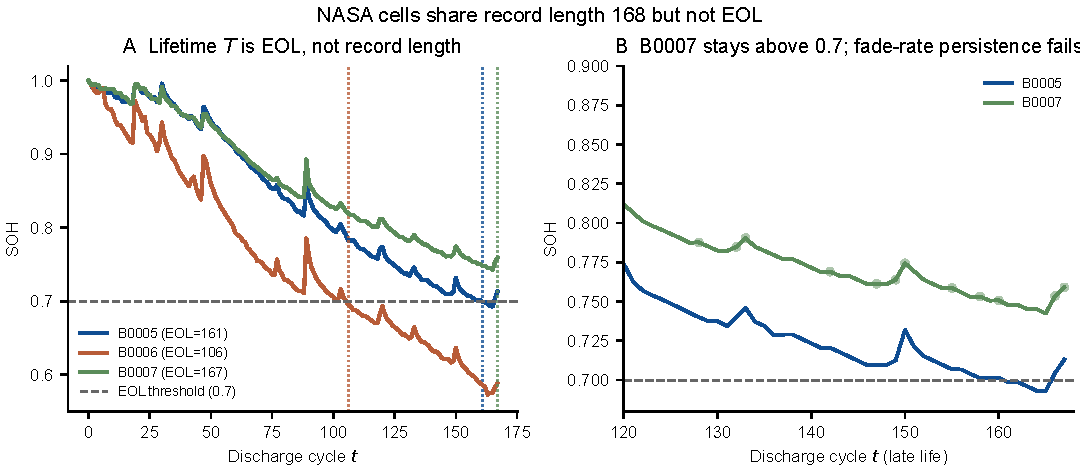
\includegraphics[width=0.98\linewidth]{fig_soh_trajectories.pdf}
\caption{NASA SOH versus cycle.
(A)~Record length is 168 for all three cells; vertical dotted lines mark $T_{\mathrm{EOL}}$.
(B)~Late-life B0007 remains above 0.7 with frequent upward ticks; constant-fade persistence then infers a near-flat slope and a large remaining life.}
\label{fig:soh}
\end{figure}

\subsection{Severson Protocol~B (primary evidence)}
\label{sec:severson}

This subsection is the primary evidence.
On Severson~\cite{severson2019nature} a stratified short/mid/long subset ($n{=}24$; $T$ from 147 to 1933) is scored with MLP under both fit protocols, with L1/L1P from the full leave-target sibling pool (Braatz exclusions; $T$ at published 80\% of nominal 1.1\,Ah).
Protocol~B is the primary leave-target-cell-out evidence (Fig.~\ref{fig:seversonb}; Table~\ref{tab:severson}); Protocol~A is the same late-20\% test windows under within-cell retrospective fitting (Table~\ref{tab:severson_A}).
Cross-cell median RUL RMSE under Protocol~B is $222.1$ (L0), $33.5$ (L1), $30.3$ (L1P), and $12.0$ (L2).
Paired Wilcoxon on $e_i=\mathrm{RMSE}_{L0,i}-\mathrm{RMSE}_{L2,i}$ gives $p=1.2{\times}10^{-7}$; L0 exceeds L2 on every scored cell.
Named L0 baselines on the same test windows (Table~\ref{tab:severson_base}) give median persist\_fade $242.8$ and persist\_recursive $499.4$; persist\_hold remains $1.0$ (oracle label walk).
MLP L0 ($222.1$) is therefore in the same regime as persist\_fade, while L2 ($12.0$) is not explained by a trivial fade foil.
Relative to Protocol~A on the same cells (Table~\ref{tab:severson_A}: L2/L1/L1P/L0 medians $15.9$/$16.9$/$19.0$/$73.4$), removing target-cell training labels widens the L0--L2 gap.
Under Protocol~B, input affinity~\eqref{eq:affine} no longer yields L1$\approx$L2 in RMSE: a constant population clock does not restore the target-specific relative-life scale across $T\in[147,1933]$.
Absolute cycle index is non-comparable across heterogeneous lifetimes; $t/T_{\mathrm{target}}$ restores that scale as a deliberate retrospective oracle (information-inconsistent only under an online-valid claim).
L1P remains the non-affine diagnostic outside~\eqref{eq:nested} (Table~\ref{tab:severson_cells}); importantly, its median error ($30.3$) is \emph{above} L2 ($12.0$) here, so the inversion reported next is protocol-specific.

\begin{figure}[htbp]
\centering
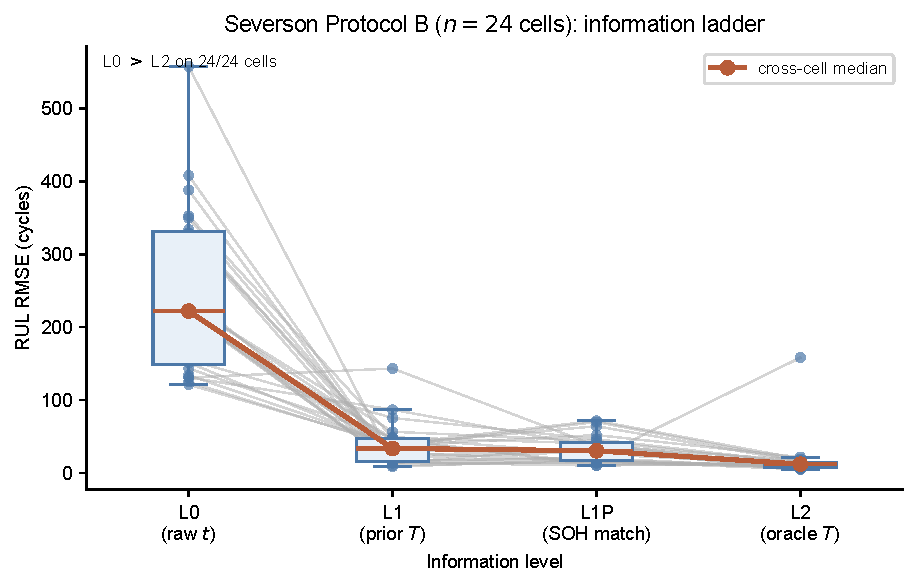
\includegraphics[width=0.98\linewidth]{fig_severson_protocol_b.pdf}
\caption{Severson Protocol~B information ladder (primary evidence; $n{=}24$ stratified cells).
Per-cell MLP trajectories with boxplots and cross-cell median overlay.
Medians: L0 $222.1$, L1 $33.5$, L1P $30.3$, L2 $12.0$ cycles.
L0$>$L2 on every scored cell (paired Wilcoxon $p=1.2{\times}10^{-7}$).}
\label{fig:seversonb}
\end{figure}

% auto-generated Severson Protocol A/B summary
\begin{table}[htbp]
\centering
\caption{Severson Protocol~A within-cell retrospective evaluation (chronological fit; MLP; stratified 24 cells; leave-target $T^{\mathrm{prior}}$ only). Cross-cell median RUL RMSE (cycles). Support comparison.}
\label{tab:severson_A}
\begin{tabular}{@{}lcccc@{}}
\toprule
Fit & L2 & L1 & L1P & L0 \\
\midrule
Protocol~A ($n=24$) & 15.9 & 16.9 & 19.0 & 73.4 \\
\bottomrule
\end{tabular}
\end{table}

\begin{table}[htbp]
\centering
\caption{Severson Protocol~B strict leave-target-cell-out evidence (MLP; same stratified 24 cells and same late-20\% test windows; train/val on sibling cells only; L1/L1P from the leave-target 119-cell pool). Cross-cell median RUL RMSE (cycles). Main evidence.}
\label{tab:severson}
\begin{tabular}{@{}lcccc@{}}
\toprule
Fit & L2 & L1 & L1P & L0 \\
\midrule
Protocol~B ($n=24$) & 12.0 & 33.5 & 30.3 & 222.1 \\
\bottomrule
\end{tabular}
\end{table}

\begin{table}[htbp]
\centering
\caption{Severson L0-valid classical foils on the same late-20\% test windows as Protocol~B ($n=24$). Cross-cell median RUL RMSE (cycles). persist\_hold $=1$ is an oracle label walk, not an L0 foil.}
\label{tab:severson_base}
\begin{tabular}{@{}lccc@{}}
\toprule
Baseline & persist\_fade & linear & persist\_recursive \\
\midrule
Protocol~B test windows & 242.8 & 228.2 & 499.4 \\
\bottomrule
\end{tabular}
\end{table}

% Protocol A Wilcoxon L0 vs L2: p=1.1920928955078125e-07, frac=1.00
% Protocol B Wilcoxon L0 vs L2: p=1.1920928955078125e-07, frac=1.00
% Protocol B classical medians: {'persist_fade': 242.77778588407944, 'linear': 228.2162851240011, 'persist_recursive': 499.3628845214844, 'persist_hold': 1.0, 'persist_mean': 299.36610154957066}
\begin{table}[htbp]
\centering
\footnotesize
\caption{Severson Protocol~B per-cell MLP RUL RMSE excerpt (mean over three seeds). Short / mid / long $T$ strata.}
\label{tab:severson_cells}
\begin{tabular}{@{}lcccc@{}}
\toprule
Cell & L2 & L1 & L1P & L0 \\
\midrule
b2c1 & 158.2 & 17.1 & 20.5 & 557.7 \\
b2c0 & 13.7 & 14.3 & 10.0 & 408.1 \\
b2c3 & 10.4 & 10.3 & 15.1 & 388.0 \\
b2c47 & 8.0 & 13.5 & 36.0 & 219.0 \\
b1c15 & 4.9 & 27.7 & 16.3 & 215.0 \\
b1c32 & 8.4 & 13.3 & 13.5 & 225.2 \\
b3c45 & 15.4 & 39.0 & 64.0 & 133.8 \\
b3c7 & 21.6 & 37.2 & 51.9 & 124.9 \\
b3c38 & 19.0 & 39.3 & 71.6 & 121.2 \\
\bottomrule
\end{tabular}
\end{table}

\subsection{Why L1P can beat L2: support, not information}
\label{sec:mechanism}

Table~\ref{tab:ladder} and Fig.~\ref{fig:l1pnasa} report the inversion: on NASA Protocol~A, MLP L1P RMSE is $5.06\pm0.23$ (B0005), $5.45\pm0.45$ (B0006), and $8.66\pm0.10$ (B0007), against L2 $23.58\pm3.85$, $10.62\pm1.69$, and $20.19\pm3.80$; Patch-TF reproduces the ordering (B0005: $2.84$ vs.\ $19.17$).
The first concern is a matching artefact, and it is excluded: the mean absolute SOH matching distance is $0.0039$ (B0005), $0.0307$ (B0006), and $0.0010$ (B0007), so the sibling lookup is local.
The second concern is that L1P secretly uses more information; it does not: the target SOH trajectory is truncated at~$t$, and neither $T_{\mathrm{target}}$ nor future SOH enters Eq.~\eqref{eq:l1p}.
The remaining question is why a channel with \emph{less} target-life information produces a lower error.

\paragraph{The oracle clock is sufficient but not learnable here.}
Under first-EOL labels, $\mathrm{RUL}=T(1-c^{(2)})$, so a linear readout of the L2 channel recovers RUL exactly; the appendix OLS check reports zero error for raw~$t$ on NASA and CALCE.
The information is therefore present; the failure is in the fitted predictor.
Because Protocol~A splits windows chronologically, every scored test window has $c^{(2)}>\max C_2$ (Section~\ref{sec:levels}): the network never sees the late-life segment of the clock during training.
On that out-of-support segment the MLP response compresses (prediction s.d.\ $0.42$--$0.50$ of the true s.d.) and over-predicts RUL by $10$--$23$ cycles, with a signed-error slope of $107$--$166$ cycles per unit of $c^{(2)}$ beyond the training maximum (Table~\ref{tab:mechanism}, Fig.~\ref{fig:mechanism}B).
The error is largest exactly where it matters for maintenance: for $\mathrm{RUL}<10$, L2 RMSE reaches $28$--$30$ cycles, while L1P is $6$--$13$ (Fig.~\ref{fig:mechanism}C).
This is the sense in which “more information” did not help: the extra information was present in the channel but outside the region where the learner could use it.

\paragraph{The local prior is interpolation, and its residual says so.}
L1P is indexed by the target's current SOH, not by cycle progress, so its lookup remains inside the sibling SOH range even when the cycle clock has left its training support.
At test, L1P is biased upward by $4.4$--$7.9$ cycles, roughly half the L2 bias, and its absolute error correlates with the SOH matching distance on the scored windows ($r=0.75$, $0.76$, $0.27$).
The pooled correlation over a whole trajectory is negative ($-0.53$, $-0.59$, $-0.10$) because early-life windows combine a tight SOH match with a large absolute RUL; conditioning on the evaluated late-life band reverses the sign.
L1P is also not a trivial copy of its channel: the prior alone has RMSE $7.25$ (B0005), $3.26$ (B0006), and $23.61$ (B0007), while the fitted model reaches $5.06$, $5.46$, and $8.66$, so the shared trunk uses the SOH trajectory to correct the prior (most visibly on censored B0007).

\paragraph{Boundary conditions.}
The inversion requires three things at once: (i)~Protocol~A, so that the target's early trajectory is in the training set; (ii)~an oracle clock whose scored values lie outside its training support; and (iii)~a sibling pool whose SOH range covers the target's late-life SOH.
Remove any one and the inversion disappears.
Under Protocol~B, L1P ($30.3$) is worse than L2 ($12.0$), because a population prior cannot recover a target-specific lifetime scale across heterogeneous cells.
On CALCE, CS2\_36 reverses the NASA order (L1P $60.69$ vs.\ L2 $2.20$), because the CALCE sibling SOH--RUL relation is not locally stable under strong regeneration.
L1P is therefore a diagnostic of local population structure, not a default online estimator.

\paragraph{Implication for online BMS.}
When $T$ is unknown, a progress clock cannot be used at all; among the online-valid options, an SOH-indexed fleet prior is a safer plug-in than an uncalibrated extrapolation of cycle progress, provided that a comparable fleet exists and its SOH coverage overlaps the target's operating range.
If no such fleet exists, the L0 recursive walk remains the fallback, and the L2 oracle should be reported only as a retrospective upper bound.
This is a use-case statement, not a claim that L1P dominates L2 in general.

\begin{table}[htbp]
\centering
\small
\caption{Error structure of the L1P inversion (NASA Protocol~A; test windows, three seeds pooled). Bias is $\mathrm{mean}(\hat y-y)$ in cycles. “s.d.\ ratio” is $\mathrm{s.d.}(\hat y)/\mathrm{s.d.}(y)$ for L2 on the scored windows; values below one indicate a compressed response. The last column is the Pearson correlation between the L1P SOH matching distance and its absolute error on the scored windows.}
\label{tab:mechanism}
\begin{tabular}{@{}lrrrrrr@{}}
\toprule
Cell & L2 RMSE & L2 bias & L2 s.d.\ ratio & L1P RMSE & L1P bias & $r(\mathrm{dist},|e|)$ \\
\midrule
B0005 & 23.79 & $+22.60$ & 0.50 & 5.06 & $+4.38$ & 0.75 \\
B0006 & 10.70 & $+10.01$ & 0.42 & 5.46 & $+5.18$ & 0.76 \\
B0007 & 20.43 & $+19.05$ & 0.50 & 8.66 & $+7.93$ & 0.27 \\
\bottomrule
\end{tabular}
\end{table}

\begin{figure}[htbp]
\centering
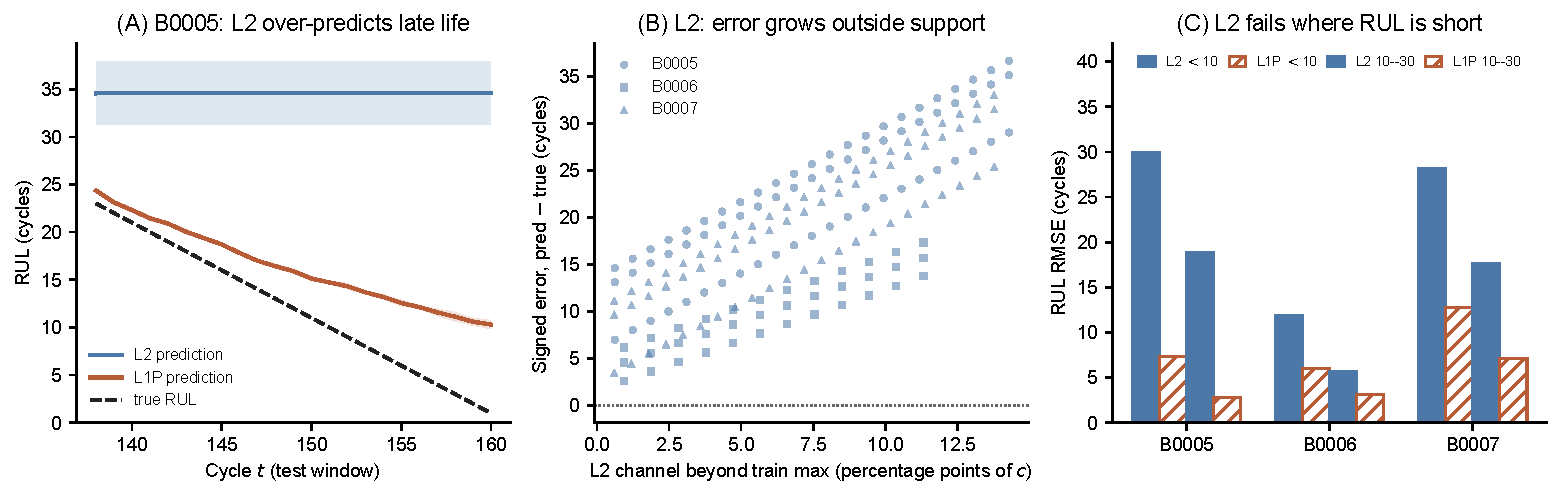
\includegraphics[width=0.99\linewidth]{fig_l1p_mechanism.pdf}
\caption{Mechanism of the L1P inversion (NASA Protocol~A; MLP, three seeds).
(A)~On B0005 the L2 prediction is nearly flat at $\sim 35$ cycles while the true RUL falls to zero; the band is $\pm$1 s.d.\ over seeds.
(B)~L2 signed error grows with the distance of the scored channel value beyond its training maximum, for all three cells.
(C)~L2 error is largest for short RUL, the regime that matters for maintenance.}
\label{fig:mechanism}
\end{figure}

\begin{figure}[htbp]
\centering
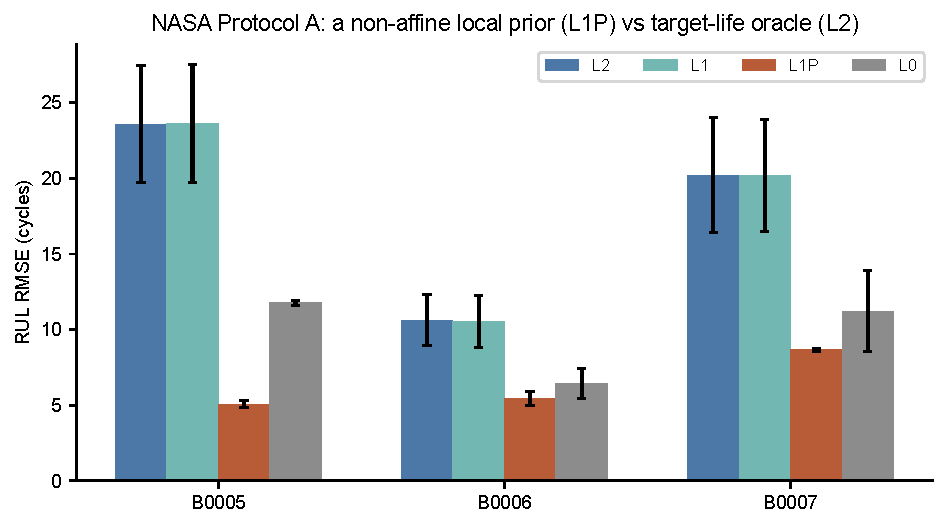
\includegraphics[width=0.98\linewidth]{fig_l1p_nasa.pdf}
\caption{NASA Protocol~A L1P versus L0/L1/L2 (MLP mean RMSE).
L1P undershoots L2 on all three cells (e.g.\ B0005: $5.06$ vs.\ $23.58$); Section~\ref{sec:mechanism} traces this to the out-of-support L2 clock rather than to a failure of the information hierarchy.}
\label{fig:l1pnasa}
\end{figure}

\subsection{Protocol sensitivity: NASA/CALCE ladder (exploratory)}
\label{sec:ladder}

This subsection demonstrates how rankings move with the fit protocol; it is \emph{not} evidence for the information hierarchy and is not pooled with Severson.
Figure~\ref{fig:ladder} and Table~\ref{tab:ladder} report re-training with $T:=T_{\mathrm{EOL}}$, L0 $=$ raw $t$, pre-EOL windows only, and B0006 included.
L1 and L2 \emph{denominators} are distinct (Table~\ref{tab:life}); RMSE need not follow the same staircase.

On NASA under Protocol~A, L1 and L2 RUL RMSE agree to two decimals for Patch-TF (e.g.\ B0005: both $19.17\pm2.42$).
This is consistent with input affinity~\eqref{eq:affine} plus empirical scale robustness (Section~\ref{sec:controls}), not a proof that $T^{\mathrm{prior}}$ was learned as a lifetime scale.
Raw-$t$ L0 is often easier on this within-cell retrospective split (Patch-TF B0005 $10.21\pm1.21$; B0006 $4.63\pm0.33$; MLP B0005 L0 $11.77\pm0.15$ vs.\ L2 $23.58\pm3.85$): the late-life test set satisfies $\mathrm{RUL}\approx c-t$, so unscaled~$t$ can match the label without an oracle denominator.
The L0-drop result in Section~\ref{sec:legacy} shows that \emph{removing} the cycle channel collapses accuracy; rescaling~$t$ does not.
Because $\mathrm{RUL}=T-t$, an on-window OLS identity check recovers $T$ algebraically from raw~$t$; this is not treated as a predictive baseline (Appendix Table~\ref{tab:clock}).
L1P breaks affine equivalence with L2 ($\rho(\mathrm{L1P},\mathrm{L2})$ from $-0.12$ to $-0.82$).
For B0005, $\mathrm{median}(T_{\mathrm{all}})=161=T_{\mathrm{target}}$ while $T^{\mathrm{prior}}=136.5$, so pooling the test cell into the prior would collapse L1 toward L2 by construction.

On CALCE the same diagnostic is not a staircase: CS2\_36 L1P is $60.69\pm20.40$ versus L2 $2.20\pm1.30$ and L0 $40.33\pm2.14$ (Table~\ref{tab:ladder}).
Hence $\operatorname{Rank}_{L1P}$ can differ from $\operatorname{Rank}_{L2}$ without a universal $\mathrm{L2}\prec\mathrm{L1P}\prec\mathrm{L0}$ order.
With first-EOL labels, CS2\_35--38 show affine L1 tracking L2 while raw-$t$ L0 is harder (e.g.\ CS2\_36: L1 $2.28\pm1.12$, L2 $2.20\pm1.30$, L0 $40.3\pm2.1$).
Patch-TF on the two-channel CALCE extract is not a reliable architecture ranking; we report it as a matched run, not as a winner.

Across seven cells, paired Wilcoxon on MLP $e_i=\mathrm{RMSE}_{L0,i}-\mathrm{RMSE}_{L2,i}$ gives $p=0.219$ (Table~\ref{tab:cellstat}): NASA L0 is easier, CALCE L0 is harder, so there is no single cell-population staircase.
This null result is expected under the design: Protocol~A asks a within-cell question, and the seven cells mix two corpora with opposite late-life behaviour.
It is reported as a descriptive sensitivity check; the primary cell-level contrast remains Severson Protocol~B (Section~\ref{sec:severson}).
Seed-level Wilcoxon tests (Table~\ref{tab:stats}, Appendix) have $n=3$ and are not used for inference.

% auto-generated; do not edit by hand
\begin{table}[htbp]
\centering
\caption{Information ladder RUL RMSE (cycles; mean$\pm$s.d.\ over three seeds). $T$ is the EOL cycle (SOH$\le 0.7$). L0 uses raw $t$. L1 uses $t/T^{\mathrm{prior}}$ from leave-target training cells. L1P is MLP only: SOH-matched sibling RUL.}
\label{tab:ladder}
\begin{tabular}{@{}llcccc@{}}
\toprule
Model & Cell & L2 & L1 & L1P & L0 \\
\midrule
\multicolumn{6}{l}{\textit{NASA}} \\
mlp & B0005 & 23.58$\pm$3.85 & 23.62$\pm$3.89 & 5.06$\pm$0.23 & 11.77$\pm$0.15 \\
mlp & B0006 & 10.62$\pm$1.69 & 10.52$\pm$1.70 & 5.45$\pm$0.45 & 6.46$\pm$0.99 \\
mlp & B0007 & 20.19$\pm$3.80 & 20.16$\pm$3.70 & 8.66$\pm$0.10 & 11.22$\pm$2.68 \\
patch-tf & B0005 & 19.17$\pm$2.43 & 19.17$\pm$2.42 & 2.84$\pm$0.89 & 10.21$\pm$1.21 \\
patch-tf & B0006 & 10.11$\pm$0.23 & 10.11$\pm$0.23 & 3.10$\pm$0.19 & 4.63$\pm$0.33 \\
patch-tf & B0007 & 15.25$\pm$2.27 & 15.26$\pm$2.27 & 3.62$\pm$0.73 & 10.84$\pm$2.08 \\
\multicolumn{6}{l}{\textit{CALCE}} \\
mlp & CS2\_35 & 2.73$\pm$1.38 & 3.00$\pm$2.15 & 18.19$\pm$9.40 & 33.42$\pm$2.78 \\
mlp & CS2\_36 & 2.20$\pm$1.30 & 2.28$\pm$1.12 & 60.69$\pm$20.40 & 40.33$\pm$2.14 \\
mlp & CS2\_37 & 2.72$\pm$1.00 & 2.86$\pm$1.11 & 15.68$\pm$0.97 & 45.28$\pm$2.45 \\
mlp & CS2\_38 & 11.87$\pm$1.95 & 12.40$\pm$1.60 & 53.74$\pm$3.25 & 46.00$\pm$3.99 \\
patch-tf & CS2\_35 & 24.85$\pm$12.20 & 32.00$\pm$4.12 & 13.25$\pm$0.63 & 23.80$\pm$3.12 \\
patch-tf & CS2\_36 & 33.74$\pm$9.75 & 41.34$\pm$0.95 & 23.33$\pm$5.26 & 27.05$\pm$6.08 \\
patch-tf & CS2\_37 & 34.65$\pm$7.25 & 35.74$\pm$0.78 & 24.51$\pm$6.81 & 26.11$\pm$10.75 \\
patch-tf & CS2\_38 & 41.56$\pm$12.26 & 25.31$\pm$9.90 & 40.66$\pm$9.34 & 28.93$\pm$2.13 \\
\bottomrule
\end{tabular}
\end{table}

\begin{table}[htbp]
\centering
\caption{Classical RUL baselines on chronological test windows with RUL$>0$. persist\_fade: SOH fade in the window (L0-valid). persist\_recursive: $\widehat{\mathrm{RUL}}_t=\max(\widehat{\mathrm{RUL}}_{t-1}-1,0)$ initialized by persist\_fade (no labels). persist\_hold uses true $\mathrm{RUL}_{t-1}$ and is an oracle walk, not an L0 BMS baseline. linear: least-squares SOH fit. Fade RMSE $>500$ is marked unstable.}
\label{tab:persist}
\begin{tabular}{@{}llcccc@{}}
\toprule
Corpus & Cell & fade & recursive & hold (oracle) & linear \\
\midrule
calce & CS2\_35 & unstable & 5.07 & 1.00 & 123.37 \\
calce & CS2\_36 & unstable & 262.71 & 1.00 & 47.55 \\
calce & CS2\_37 & unstable & 7.83 & 1.00 & 79.85 \\
calce & CS2\_38 & unstable & 265.78 & 1.00 & 308.31 \\
nasa & B0005 & 7.63 & 6.14 & 1.00 & 7.92 \\
nasa & B0006 & 3.68 & 0.48 & 1.00 & 7.33 \\
nasa & B0007 & 30.29 & 15.53 & 1.00 & 28.10 \\
\bottomrule
\end{tabular}
\end{table}

\begin{table}[htbp]
\centering
\caption{Cell-level MLP RUL RMSE (mean over three seeds). The experimental unit is the cell ($n{=}7$). Paired Wilcoxon on $\mathrm{RMSE}_{L0}-\mathrm{RMSE}_{L2}$: $p=0.219$; on $\mathrm{RMSE}_{L1}-\mathrm{RMSE}_{L2}$: $p=0.156$. Signs mix across NASA (L0 easier) and CALCE (L0 harder); seed tests are not a substitute.}
\label{tab:cellstat}
\begin{tabular}{@{}llccc@{}}
\toprule
Corpus & Cell & L2 & L1 & L0 \\
\midrule
calce & CS2\_35 & 2.73 & 3.00 & 33.42 \\
calce & CS2\_36 & 2.20 & 2.28 & 40.33 \\
calce & CS2\_37 & 2.72 & 2.86 & 45.28 \\
calce & CS2\_38 & 11.87 & 12.40 & 46.00 \\
nasa & B0005 & 23.58 & 23.62 & 11.77 \\
nasa & B0006 & 10.62 & 10.52 & 6.46 \\
nasa & B0007 & 20.19 & 20.16 & 11.22 \\
\bottomrule
\end{tabular}
\end{table}

\begin{figure}[htbp]
\centering
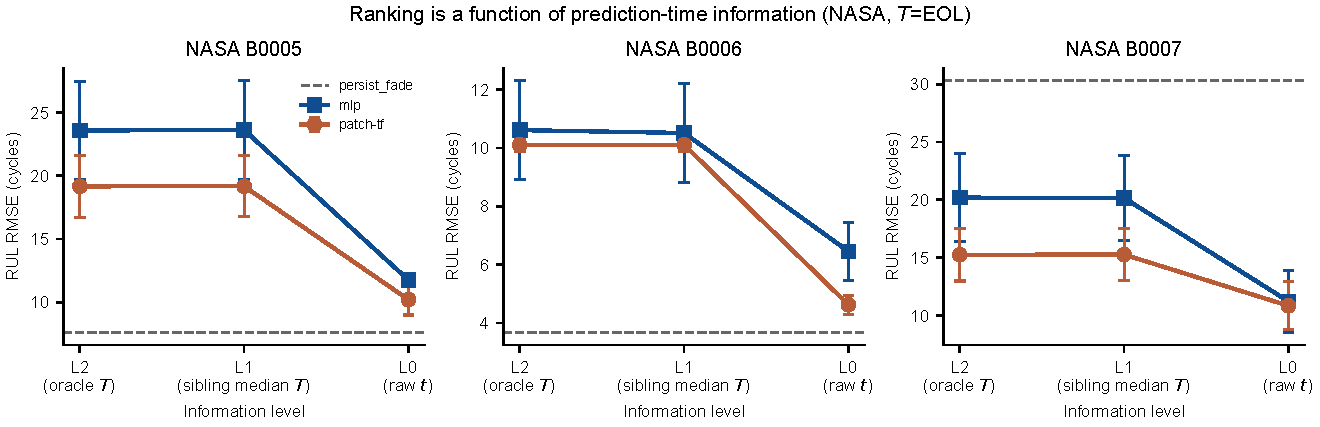
\includegraphics[width=0.98\linewidth]{fig_info_levels.pdf}
\caption{NASA Protocol~A exploratory ladder (mean$\pm$s.d., three seeds).
Dashed line: persist\_fade.
L1 uses leave-target-out median $T_{\mathrm{EOL}}$.
L1 and L2 traces overlap; raw-$t$ L0 is a same-cell countdown.}
\label{fig:ladder}
\end{figure}

\begin{figure}[htbp]
\centering
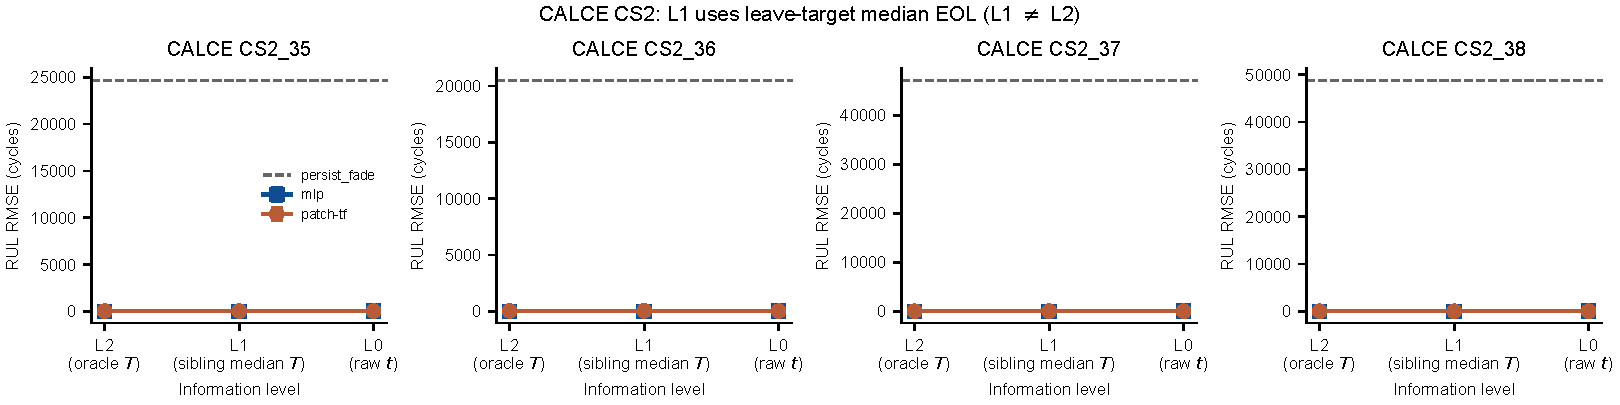
\includegraphics[width=0.98\linewidth]{fig_info_levels_calce.pdf}
\caption{CALCE CS2 exploratory ladder (demoted relative to Severson Protocol~B).
MLP on CS2\_36--38 shows L2$\approx$L1 $\ll$ L0; persist\_fade (dashed) explodes under regeneration.}
\label{fig:laddercalce}
\end{figure}

\subsection{Revision controls: scale, matching, SOH heads, support}
\label{sec:controls}

Four controls bound the mechanism in Section~\ref{sec:mechanism} (artifacts in \path{outputs/revision_controls/} and \path{outputs/l1p_mechanism/}).

\paragraph{Scale control.}
An independent matched MLP re-run (seeds $\{42,43,44\}$; same Protocol~A windows; not the Table~\ref{tab:ladder} training run) isolates numerical scale from the lifetime label.
In that re-run, L1 and L2 RUL RMSE agree to within $\sim 0.1$ cycle (B0005: $23.62\pm3.17$ vs.\ $23.58\pm3.15$; similarly B0006/B0007), while raw-$t$ L0 is lower on B0005 ($14.92\pm1.48$) and B0007 ($13.58\pm2.76$).
An L0 clock $t/1000$ recovers L1/L2-like errors ($23.11\pm3.07$ on B0005).
Means for L2 match Table~\ref{tab:ladder} to two decimals; seed-wise s.d.\ and L0 means differ because the runs are not identical, so scale-control numbers must not be mixed with Table~\ref{tab:ladder} as one estimate.
This control indicates that the L1/L2 behaviour is partly attributable to numerical scale rather than to the semantic meaning of the lifetime constant alone.
Pointwise $|\hat y^{\mathrm{L1}}-\hat y^{\mathrm{L2}}|$ has mean $<0.25$ cycle and correlation $>0.97$ across seeds, supporting empirical scale robustness without claiming invariance.

\paragraph{Channel support.}
On every scored NASA test window, the L2 channel lies above its training maximum: $c^{(2)}$ test ranges are $0.85$--$0.99$ (B0005), $0.89$--$0.99$ (B0006), and $0.83$--$0.97$ (B0007), against training maxima $0.85$, $0.88$, and $0.83$.
The same holds for window-interior values (the often-cited “24\% above train max” counts cycles inside test windows, not window-end values, and understates the issue).
L1 and L0 are monotone in~$t$ and inherit the same out-of-support status, but their numerical ranges differ; raw~$t$ happens to extrapolate better than the compressed clock $c^{(2)}$, which is a scale effect rather than an information effect.
This is why Section~\ref{sec:mechanism} reads the L2 failure as learnability, not as insufficiency.

\paragraph{L1P matching distance.}
Mean absolute SOH matching distances are small (B0005 $0.0039$; B0006 $0.0307$; B0007 $0.0010$), so L1P undershoot of L2 is not an artifact of failed nearest-neighbour SOH lookup.
Over full trajectories the correlation between matching distance and absolute RUL error is weak-to-negative (B0005 $-0.53$; B0006 $-0.59$; B0007 $-0.10$) because early-life windows combine tight matches with large absolute RUL.
On the scored late-life windows the sign reverses ($0.75$, $0.76$, $0.27$; Table~\ref{tab:mechanism}), which is the relevant check: where L1P is used, a poorer SOH match does predict a larger error.

\paragraph{SOH-only versus dual-head (healthy default).}
Table~\ref{tab:sohcontrol} is the dual-head health check that motivates the default objective.
Under the unnormalised ablation $\mathcal{L}_{\mathrm{SOH}}+0.5\,\mathcal{L}_{\mathrm{RUL}}$, SOH RMSE is $0.56$--$0.81$ while an SOH-only head on the same windows reaches $0.017$--$0.031$; $g_{\mathrm{RUL}}/g_{\mathrm{SOH}}$ at the shared trunk is $64$--$130$, and early stopping is driven by validation RUL RMSE.
The SOH head is therefore under-trained, not unlearnable.
Under the \textbf{default} normalised loss $\mathcal{L}_{\mathrm{SOH}}+0.5\,\mathcal{L}_{\mathrm{RUL}/T}$, SOH RMSE recovers to $0.026$--$0.177$ (near the SOH-only floor), while RUL RMSE moves by at most $\sim 5$ cycles (B0005 L2: $23.58\to 19.43$) and leaves every hierarchy ordering in this paper unchanged---including L1P$<$L2 on NASA Protocol~A and L0$\gg$L2 on Severson Protocol~B.
The information-level conclusions therefore hold under a dual-head configuration whose SOH head is no longer pathological.
The full per-level dual-head table remains Appendix-only (Table~\ref{tab:soh}) as a multi-task diagnostic, not an SOH benchmark.

\begin{table}[htbp]
\centering
\footnotesize
\caption{Dual-head health check under NASA Protocol~A, L2 channel (three seeds, mean$\pm$s.d.).
``Ablation'' is $\mathcal{L}_{\mathrm{SOH}}+0.5\mathcal{L}_{\mathrm{RUL}}$; ``Default (norm.)'' is $\mathcal{L}_{\mathrm{SOH}}+0.5\mathcal{L}_{\mathrm{RUL}/T}$; ``SOH-only'' early-stops on SOH RMSE.
Last column: $g_{\mathrm{RUL}}/g_{\mathrm{SOH}}$ under the ablation (first three epochs).
Default RUL columns are the healthy-model supplement to the main L2 ranking numbers.}
\label{tab:sohcontrol}
\setlength{\tabcolsep}{2pt}
\begin{tabular}{@{}lcccccc@{}}
\toprule
Cell & SOH (abl.) & SOH (def.) & SOH-only & RUL (abl.) & RUL (def.) & $g_{\mathrm{RUL}}/g_{\mathrm{SOH}}$ \\
\midrule
B0005 & $0.706\pm0.184$ & $0.034\pm0.022$ & $0.017\pm0.002$ & $23.58\pm3.85$ & $19.43\pm6.36$ & 124 \\
B0006 & $0.812\pm0.294$ & $0.177\pm0.060$ & $0.031\pm0.005$ & $10.62\pm1.69$ & $15.42\pm7.94$ & 64 \\
B0007 & $0.562\pm0.142$ & $0.026\pm0.014$ & $0.020\pm0.003$ & $20.19\pm3.80$ & $24.51\pm3.89$ & 130 \\
\bottomrule
\end{tabular}
\end{table}

\subsection{Legacy L2 under $T_{\mathrm{record}}$}
\label{sec:legacy}

This subsection is a historical oracle baseline under $T_{\mathrm{record}}$, not primary evidence.
Table~\ref{tab:l2legacy} restates the earlier matched chronological comparison that used $T_{\mathrm{record}}$ in $\mathrm{cycle\_norm}$.
Those numbers describe ranking when relative progress to the \emph{recorded} end is known, and when L1 cannot separate from L2.
They are not deleted; they are relabeled as an oracle with a degenerate lifetime definition.

\begin{table}[htbp]
\centering
\caption{Legacy L2 (oracle with $T=T_{\mathrm{record}}$) matched RUL RMSE (cycles; three seeds). Persistence here is persist\_fade on the untruncated chronological tail.}
\label{tab:l2legacy}
\begin{tabular}{@{}lcc@{}}
\toprule
Model & B0005 & B0007 \\
\midrule
persist\_fade & $6.81$ & $30.30$ \\
Linear extrap. & $7.01$ & $28.10$ \\
MLP & $5.22\pm0.99$ & $\mathbf{5.91\pm1.91}$ \\
Patch-TF & $\mathbf{2.28\pm0.96}$ & $9.67\pm2.95$ \\
\bottomrule
\end{tabular}
\end{table}

Dropping $\mathrm{cycle\_norm}$ while keeping the other five channels (L0-drop, same legacy split) collapsed Patch-TF and MLP to about $19$--$22$ RMSE on both cells.
That remains the sharpest single demonstration that the legacy headline error was not a property of capacity/voltage channels alone.

\subsection{Why persist\_fade fails on B0007, and why $T$ is censored}
\label{sec:b0007}

On the legacy split, persist\_fade is 6.81 cycles on B0005 and 30.3 on B0007.
Fig.~\ref{fig:soh}B shows the mechanism: B0007's recorded SOH ends near 0.76 and never crosses 0.7, so $T$ equals the last observed cycle, and late increments are often positive.
A window fade rate near zero maps to an enormous implied RUL.
The failure therefore has two coupled causes: the local fade is non-monotone, and the target is \emph{right-censored}, so extrapolating to 0.7 asks the baseline to invent a decline that was never observed.
The L0-valid recursive walk, initialized by persist\_fade then counting down by one cycle, is $15.53$ on B0007 versus $6.14$ on B0005 (Table~\ref{tab:persist}).
persist\_hold remains $1.0$ because it copies true $\mathrm{RUL}_{t-1}$ and is an oracle.
“Learned models beat persistence under L0 on B0007” is therefore true for persist\_fade ($30.29$) and must not be written against persist\_hold.
Because B0007 is censored, its absolute RUL RMSE is a record-horizon error and should not be compared numerically with B0005/B0006; it is used here as a stress case for the L1P mechanism and for persist\_fade, not as a lifetime benchmark.

\section{Discussion}
\label{sec:discussion}

\paragraph{Finding 1: information level changes the ranking.}
Under Severson Protocol~B ($n{=}24$), median MLP RMSE falls from $222.1$ at L0 to $12.0$ at L2, and L0 exceeds L2 on every scored cell (Fig.~\ref{fig:seversonb}).
That leave-target-cell-out ladder is the primary support for $\operatorname{Rank}(\cdot\mid\mathcal{I}_t)=f(\mathcal{I}_t)$.
The L0 error is in the same regime as persist\_fade ($242.8$), so the ladder is not an artefact of a weak model family.

\paragraph{Finding 2: the L1P inversion is a support-and-learnability effect.}
NASA Protocol~A adds a narrower second lesson, and the mechanism analysis sharpens it.
L1P can beat L2 even when SOH matching distances stay small (Fig.~\ref{fig:l1pnasa}), because the L2 clock is evaluated outside its training support and the fitted network compresses late-life variation, while L1P is an SOH-indexed local average that remains inside its matching neighbourhood (Section~\ref{sec:mechanism}).
This is not a case of “less information is better”.
It is a case in which additional information was \emph{sufficient but not learnable} on the scored windows under the chosen fit protocol, a distinction that a single RMSE column cannot reveal.
The inversion disappears under Protocol~B (L1P $30.3$ vs.\ L2 $12.0$) and reverses on CALCE CS2\_36 (L1P $60.69$ vs.\ L2 $2.20$), so the correct claim is conditional, not universal.

\paragraph{Finding 3: Protocol~A and Protocol~B answer different questions.}
Equation~\eqref{eq:affine} explains why L1 and L2 look alike under Protocol~A: they are affine rescalings of the same~$t$ (Table~\ref{tab:affine}).
Scale-control runs confirm empirical robustness of the trained networks, but they do not prove invariance.
Protocol~B breaks the practical L1$\approx$L2 pattern because a single sibling prior cannot restore target-specific relative life across $T\in[147,1933]$.
Under Protocol~A, raw~$t$ can also beat L2 when the late-life test set is essentially a within-cell countdown.
That pattern is a Protocol~A artifact; it does not overturn the Protocol~B result, and it is the reason Section~\ref{sec:ladder} is labelled exploratory.

\paragraph{Relation to benchmark platforms.}
BatteryML~\cite{zhang2024batteryml} and BatteryLife~\cite{tan2025batterylife} make data pipelines and model comparisons reproducible; this paper addresses a different axis, the auditability of the information condition.
The two are complementary: dataset and model cards can carry an “information level / fit protocol / $T$ definition / scaler source / support status” row for every reported score, and the ladder can be implemented as a wrapper around their evaluation harness without changing the models.
We do not claim that current platforms are leaky; we claim that their reporting cards leave the information condition implicit, which is enough for two incomparable scores to appear side by side.

\paragraph{Practical guidance.}
For an online BMS claim, L2 must be reported as a named retrospective oracle and never as a deployable result.
When $T$ is unknown and a comparable fleet exists, an SOH-indexed sibling prior is a reasonable online-valid plug-in, with the caveat that it needs SOH coverage and a stable local SOH--RUL relation; when no fleet exists, keep the L0 recursive walk and report the oracle only as an upper bound.
For a benchmark claim, report Protocol~B; for a within-cell retrospective study, report Protocol~A and state that L1/L1P may be undefined without siblings.

\paragraph{Limitations.}
NASA and CALCE stay Protocol~A diagnostics, and the mechanism analysis rests on three NASA cells.
Severson Protocol~B uses a stratified 24-cell stress subset of 119 usable cells, not a random population sample.
B0007 is right-censored, so its absolute errors are record-horizon errors.
Beyond NASA cycle aggregates, the extracts omit full in-cycle V/I/T trajectories.
All scores are cycle-level after a completed discharge.
The SOH head is a diagnostic, not a validated SOH estimator, and its repair is demonstrated only on NASA.
Finally, L1P is a local prior: it is only as good as the sibling coverage, and its failure on CALCE CS2\_36 is part of the result rather than an outlier to be removed.

\section{Conclusion}
\label{sec:conclusion}

RUL benchmarks should encode prediction-time information in the protocol itself.
Information-consistent evaluation couples four things that are usually reported separately: a named information level, a declared fit protocol, a provenance and support audit, and a fillable report row.
Under first-EOL labels and named L0/L1/L1P/L2 cycle channels, leave-target evaluation on Severson ($n{=}24$) shows that information level changes RUL error (L0 $222.1$ vs.\ L2 $12.0$; $p=1.2{\times}10^{-7}$).
NASA Protocol~A further shows a setting-specific reversal, L1P beating L2, which we trace to the oracle clock leaving its training support while an SOH-indexed local prior stays inside its matching neighbourhood.
Future tables should report information level, fit protocol, the $T$ definition and censoring status, channel support, and persist\_fade with RMSE, not the architecture name alone.

\section*{Appendix. OLS identity check}
% OLS identity check (appendix only; not a predictive baseline)
\begin{table}[htbp]
\centering
\caption{Appendix OLS identity check on evaluated chronological windows (RUL$>0$).
OLS is an algebraic diagnostic of $\mathrm{RUL}=\max(0,T-t)$, not an out-of-sample predictive baseline: it is fit with an intercept on the same scored windows.
Under that identity, OLS RMSE on raw~$t$ is numerically zero on NASA and CALCE.
$\rho$ is Pearson correlation; $\rho(\mathrm{L1},\mathrm{L2})=1$ because L1 and L2 are affine in~$t$.
L1P is not affine in~$t$.}
\label{tab:clock}
\begin{tabular}{@{}llcccc@{}}
\toprule
Corpus & Cell & $\rho(\mathrm{L1},\mathrm{L2})$ & $\rho(\mathrm{L1P},\mathrm{L2})$ & OLS $t$ & OLS L1P \\
\midrule
nasa & B0005 & 1.000 & -0.703 & 0 & 14.20 \\
nasa & B0006 & 1.000 & -0.598 & 0 & 15.57 \\
nasa & B0007 & 1.000 & -0.824 & 0 & 13.28 \\
calce & CS2\_35 & 1.000 & -0.122 & 0 & 98.18 \\
calce & CS2\_36 & 1.000 & -0.706 & 0 & 101.04 \\
calce & CS2\_37 & 1.000 & -0.654 & 0 & 99.90 \\
calce & CS2\_38 & 1.000 & -0.621 & 0 & 96.29 \\
\bottomrule
\end{tabular}
\end{table}


\section*{Appendix. Seed-level contrasts and full SOH table}
% auto-generated appendix tables (moved from generated_tables.tex)
\begin{table}[htbp]
\centering
\caption{SOH RMSE (dimensionless; mean$\pm$s.d.\ over three seeds) under the same information ladder.}
\label{tab:soh}
\begin{tabular}{@{}llccc@{}}
\toprule
Model & Cell & L2 & L1 & L0 \\
\midrule
mlp & B0005 & 0.7063$\pm$0.1843 & 0.7007$\pm$0.1826 & 0.3302$\pm$0.0660 \\
mlp & B0006 & 0.8120$\pm$0.2939 & 0.8180$\pm$0.2988 & 0.2879$\pm$0.0462 \\
mlp & B0007 & 0.5625$\pm$0.1420 & 0.5640$\pm$0.1332 & 0.3358$\pm$0.0264 \\
patch-tf & B0005 & 0.3593$\pm$0.0567 & 0.3583$\pm$0.0565 & 0.5132$\pm$0.1256 \\
patch-tf & B0006 & 0.5564$\pm$0.3209 & 0.5548$\pm$0.3199 & 0.4427$\pm$0.0678 \\
patch-tf & B0007 & 0.4028$\pm$0.0108 & 0.4044$\pm$0.0119 & 0.6538$\pm$0.4076 \\
\bottomrule
\end{tabular}
\end{table}

\begin{table}[htbp]
\centering
\caption{Seed-level paired contrasts of RUL RMSE (selected). The experimental unit is the random seed on a fixed cell ($n=3$), not the cell. Wilcoxon $p{=}0.25$ is the smallest two-sided value when all three seeds move in the same direction. Full contrasts are in \texttt{outputs/info\_levels\_v2/stats.json}.}
\label{tab:stats}
\begin{tabular}{@{}llllccc@{}}
\toprule
Contrast & Corpus & Model & Cell & $\Delta$RMSE & Cohen's $d$ & $p$ \\
\midrule
L2-vs-L0 & calce & mlp & CS2\_35 & 30.69 & 13.98 & 0.250 \\
L2-vs-L1 & calce & mlp & CS2\_35 & 0.27 & 0.15 & 0.750 \\
L2-vs-L0 & calce & mlp & CS2\_36 & 38.13 & 21.52 & 0.250 \\
L2-vs-L1 & calce & mlp & CS2\_36 & 0.08 & 0.07 & 0.750 \\
L2-vs-L0 & calce & mlp & CS2\_37 & 42.55 & 22.73 & 0.250 \\
L2-vs-L1 & calce & mlp & CS2\_37 & 0.14 & 0.13 & 0.500 \\
L2-vs-L0 & calce & mlp & CS2\_38 & 34.13 & 10.86 & 0.250 \\
L2-vs-L1 & calce & mlp & CS2\_38 & 0.53 & 0.30 & 0.500 \\
L2-vs-L0 & nasa & mlp & B0005 & -11.81 & -4.33 & 0.250 \\
L2-vs-L1 & nasa & mlp & B0005 & 0.04 & 0.01 & 0.750 \\
L2-vs-L0 & nasa & mlp & B0006 & -4.16 & -3.00 & 0.250 \\
L2-vs-L1 & nasa & mlp & B0006 & -0.10 & -0.06 & 0.250 \\
L2-vs-L0 & nasa & mlp & B0007 & -8.97 & -2.73 & 0.250 \\
L2-vs-L1 & nasa & mlp & B0007 & -0.03 & -0.01 & 1.000 \\
L2-vs-L0 & nasa & patch-tf & B0005 & -8.95 & -4.67 & 0.250 \\
L2-vs-L1 & nasa & patch-tf & B0005 & 0.01 & 0.00 & 1.000 \\
L2-vs-L0 & nasa & patch-tf & B0006 & -5.49 & -19.33 & 0.250 \\
L2-vs-L1 & nasa & patch-tf & B0006 & -0.01 & -0.03 & 0.750 \\
L2-vs-L0 & nasa & patch-tf & B0007 & -4.41 & -2.03 & 0.250 \\
L2-vs-L1 & nasa & patch-tf & B0007 & 0.02 & 0.01 & 0.500 \\
\bottomrule
\end{tabular}
\end{table}



\section*{Appendix. Reporting template}

\begin{table}[htbp]
\centering
\footnotesize
\setlength{\tabcolsep}{3pt}
\caption{Minimum report row (copy per model $\times$ cell $\times$ level).}
\label{tab:template}
\begin{tabular}{@{}p{0.14\linewidth}p{0.07\linewidth}p{0.15\linewidth}p{0.08\linewidth}p{0.08\linewidth}p{0.10\linewidth}p{0.09\linewidth}@{}}
\toprule
Model & Level & Cycle channel & $W$, $H$ & Scaler & Support & RUL RMSE \\
\midrule
Patch-TF & L0 & raw $t$ & 50, 5 & train & in & \ldots \\
Patch-TF & L1 & $t/T_{\mathrm{med}}$ & 50, 5 & train & in & \ldots \\
Patch-TF & L2 & $t/T_{\mathrm{target}}$ & 50, 5 & train & out (oracle) & \ldots \\
persist\_fade & --- & SOH only & 50, --- & --- & --- & \ldots \\
\bottomrule
\end{tabular}
\end{table}

Required fields: corpus, cell id, $T$ definition and whether EOL was reached, whether post-EOL windows are dropped, persist\_fade RMSE, fit protocol, channel support status, and the information level of every learned row.
Optional: SOH RMSE as an auxiliary control; PICP/PINAW in the appendix.

\section*{Appendix. Uncertainty (not a calibration claim)}
% auto-generated UQ appendix; do not edit by hand
\begin{table}[htbp]
\centering
\caption{Appendix. MC-Dropout 95\% intervals ($n_{\mathrm{MC}}=20$) for Patch-TF RUL on NASA. PICP is empirical coverage of mean$\pm 1.96$ std; PINAW is width normalized by the test RUL range. Not used as a calibration claim.}
\label{tab:uq}
\begin{tabular}{@{}lcccc@{}}
\toprule
Cell & L2 PICP & L2 PINAW & L0 PICP & L0 PINAW \\
\midrule
B0005 & 0.058$\pm$0.025 & 0.599$\pm$0.077 & 0.522$\pm$0.174 & 0.879$\pm$0.167 \\
B0006 & 0.056$\pm$0.048 & 0.709$\pm$0.041 & 0.528$\pm$0.210 & 0.878$\pm$0.265 \\
B0007 & 0.217$\pm$0.075 & 0.607$\pm$0.097 & 0.377$\pm$0.280 & 0.792$\pm$0.165 \\
\bottomrule
\end{tabular}
\end{table}


\section*{Statements and Declarations}
\paragraph{Funding.} None.
\paragraph{Competing interests.} None.
\paragraph{Data availability.}
NASA PCoE cells B0005--B0007~\cite{saha2007nasa}; CALCE CS2 cells~\cite{he2011calce}; Severson/MATR batches~\cite{severson2019nature}.
Replication scripts and adopted experiment outputs: \path{scripts/run_info_levels_v2.py}, \path{scripts/run_revision_controls.py}, \path{scripts/run_l1p_mechanism.py}, \path{experiments/info_consistent/}, \path{outputs/info_levels_v2/}, \path{outputs/info_levels_severson_loco/}, \path{outputs/revision_controls/}, \path{outputs/l1p_mechanism/}.
A versioned code bundle is maintained in the project git repository; the public GitHub URL and Zenodo DOI will be inserted here upon first deposit (see \path{CODE_AVAILABILITY.md}).

\begin{thebibliography}{99}

%% ---- foundational corpora / protocol anchors (pre-2025 minority) ----
\bibitem{saha2007nasa}
B.~Saha, K.~Goebel,
Battery Data Set,
NASA Ames Prognostics Data Repository,
Moffett Field, CA (2007).

\bibitem{saha2009compare}
B.~Saha, K.~Goebel, J.~Christophersen,
Comparison of prognostic algorithms for estimating remaining useful life of batteries,
Trans.\ Inst.\ Meas.\ Control 31~(3--4) (2009) 293--308.

\bibitem{he2011calce}
W.~He, N.~Williard, M.~Osterman, M.~Pecht,
Prognostics of lithium-ion batteries based on Dempster--Shafer theory and the Bayesian Monte Carlo method,
J.\ Power Sources 196~(23) (2011) 10314--10321.

\bibitem{kaufman2012leakage}
S.~Kaufman, S.~Rosset, C.~Perlich, O.~Stitelman,
Leakage in data mining: Formulation, detection, and avoidance,
ACM Trans.\ Knowl.\ Discov.\ Data 6~(4) (2012) 1--21.

\bibitem{gal2016}
Y.~Gal, Z.~Ghahramani,
Dropout as a Bayesian approximation: representing model uncertainty in deep learning,
in: Proc.\ 33rd Int.\ Conf.\ Mach.\ Learn., PMLR 48 (2016) 1050--1059.

\bibitem{vaswani2017}
A.~Vaswani, N.~Shazeer, N.~Parmar, J.~Uszkoreit, L.~Jones, A.N.~Gomez, L.~Kaiser, I.~Polosukhin,
Attention is all you need,
in: Adv.\ Neural Inf.\ Process.\ Syst.\ 30 (2017) 5998--6008.

\bibitem{birkl2017}
C.R.~Birkl, M.R.~Roberts, E.~McTurk, P.G.~Bruce, D.A.~Howey,
Degradation diagnostics for lithium ion cells,
J.\ Power Sources 341 (2017) 373--386.

\bibitem{xiong2018soh}
R.~Xiong, L.~Li, J.~Tian,
Towards a smarter battery management system: a critical review on battery state of health monitoring methods,
J.\ Power Sources 405 (2018) 18--29.

\bibitem{lipu2018}
M.S.H.~Lipu, M.A.~Hannan, A.~Hussain, M.M.~Hoque, P.J.~Ker, S.M.A.~Saad, A.~Ayob,
A review of state of health and remaining useful life estimation methods for lithium-ion battery in electric vehicles: challenges and recommendations,
J.\ Clean.\ Prod.\ 205 (2018) 115--133.

\bibitem{hu2019rser}
X.~Hu, F.~Feng, K.~Liu, L.~Zhang, J.~Xie, B.~Liu,
State estimation for advanced battery management: key challenges and future trends,
Renew.\ Sustain.\ Energy Rev.\ 114 (2019) 109334.

\bibitem{severson2019nature}
K.A.~Severson, P.M.~Attia, N.~Jin, N.~Perkins, B.~Jiang, Z.~Yang, M.H.~Chen, M.~Aykol, P.K.~Herring, D.~Fraggedakis, M.Z.~Bazant, S.J.~Harris, W.C.~Chueh, R.D.~Braatz,
Data-driven prediction of battery cycle life before capacity degradation,
Nat.\ Energy 4 (2019) 383--391.

\bibitem{roman2021}
D.~Roman, S.~Saxena, V.~Robu, M.~Pecht, D.~Flynn,
Machine learning pipeline for battery state-of-health estimation,
Nat.\ Mach.\ Intell.\ 3 (2021) 447--456.

\bibitem{sulzer2021joule}
V.~Sulzer, P.~Mohtat, A.~Aitio, S.~Lee, Y.T.~Yeh, F.~Steinbacher, M.U.~Khan, J.W.~Lee, J.B.~Siegel, A.G.~Stefanopoulou, D.A.~Howey,
The challenge and opportunity of battery lifetime prediction from field data,
Joule 5 (2021) 1934--1955.

\bibitem{geslin2023joule}
A.~Geslin, B.~van Vlijmen, X.~Cui, A.~Bhargava, P.A.~Asinger, R.D.~Braatz, W.C.~Chueh,
Selecting the appropriate features in battery lifetime predictions,
Joule 7 (2023) 1956--1965.

\bibitem{kapoor2023leakage}
S.~Kapoor, A.~Narayanan,
Leakage and the reproducibility crisis in machine-learning-based science,
Patterns 4~(9) (2023) 100804.

\bibitem{nie2023patchtst}
Y.~Nie, N.H.~Nguyen, P.~Sinthong, J.~Kalagnanam,
A time series is worth 64 words: long-term forecasting with transformers,
in: Int.\ Conf.\ Learn.\ Represent.\ (2023).

\bibitem{rosenblatt2024}
M.~Rosenblatt, L.~Tejavibulya, R.~Jiang, S.M.~Noble, D.~Scheinost,
Data leakage inflates prediction performance in connectome-based machine learning models,
Nat.\ Commun.\ 15 (2024) 1829.

\bibitem{zhang2024batteryml}
H.~Zhang, X.~Gui, S.~Zheng, Z.~Lu, Y.~Li, J.~Bian,
BatteryML: An open-source platform for machine learning on battery degradation,
in: Int.\ Conf.\ Learn.\ Represent.\ (2024).

\bibitem{li2024lifetime}
T.~Li, Z.~Zhou, A.~Thelen, D.A.~Howey, C.~Hu,
Predicting battery lifetime under varying usage conditions from early aging data,
Cell Rep.\ Phys.\ Sci.\ 5~(4) (2024) 101891.

%% ---- 2025--2026 majority ----
\bibitem{wang2024gce}
S.~Wang, R.~Zhou, Y.~Ren, M.~Jiao, H.~Liu, C.~Lian,
Advanced data-driven techniques in AI for predicting lithium-ion battery remaining useful life: a comprehensive review,
Green Chem.\ Eng.\ 6~(2) (2025) 139--153.

\bibitem{zhang2025batlinet}
H.~Zhang, Y.~Li, S.~Zheng, Z.~Lu, X.~Gui, W.~Xu, J.~Bian,
Battery lifetime prediction across diverse ageing conditions with inter-cell deep learning,
Nat.\ Mach.\ Intell.\ 7 (2025) 270--277.

\bibitem{tan2025batterylife}
R.~Tan, W.~Hong, J.~Tang, X.~Lu, R.~Ma, X.~Zheng, J.~Li, J.~Huang, T.-Y.~Zhang,
BatteryLife: A comprehensive dataset and benchmark for battery life prediction,
arXiv:2502.18807 (2025).

\bibitem{madani2025groupkfold}
S.S.~Madani, M.~H\'{e}bert, L.~Boulon, A.~Lupien-B\'{e}dard, F.~Allard,
Comparative analysis of ML and DL models for data-driven SOH estimation of LIBs under diverse temperature and load conditions,
Batteries 11~(11) (2025) 393.

\bibitem{xu2025meas}
Z.~Xu, J.~Mao, Y.~Han, H.~Yuan,
A comprehensive review of lithium-ion battery remaining useful life prediction: methodologies, datasets, performance metrics, and future perspectives,
Meas.\ Sci.\ Technol.\ 36~(8) (2025) 082001.

\bibitem{yang2025batteries}
Y.~Yang, S.~Wang, Y.~Zhou, C.~Fernandez,
A critical review of AI-based battery remaining useful life prediction for energy storage systems,
Batteries 11~(10) (2025) 376.

\bibitem{deng2025piml}
Y.~Deng, X.~Le, T.T.~Nguyen, C.~Gogu,
A generic physics-informed machine learning framework for battery remaining useful life prediction using small early-stage lifecycle data,
Appl.\ Energy 384 (2025) 125314.

\bibitem{oyewole2025uq}
I.~Oyewole, W.~Hassanieh, M.~Chelbi, A.~Chehade,
Uncertainty-aware deep learning with physics-informed bayesian sampling for lithium-ion battery prognostics,
Appl.\ Energy 402 (2025) 126880.

\bibitem{aliakbari2025fusedr}
S.~Aliakbari, M.~Masih-Tehrani,
FuseDR-Net: a fusion-based network for battery remaining useful life prediction using causally decomposed health indicators,
Energy Convers.\ Manag.\ X 28 (2025) 101341.

\bibitem{ge2025koopman}
X.~Ge, Y.~Jiang, B.~Xu,
Deep Koopman operator-based remaining useful life prediction of Lithium-ion batteries under multi-condition scenarios,
J.\ Energy Storage 119 (2025) 116369.

\bibitem{li2025adapt}
J.~Li, Z.~Wang, D.~Tian, Z.~Sun, Y.~Niu,
A novel RUL prediction framework based on the adaptability feature perception fusion model method,
J.\ Energy Storage 119 (2025) 116322.

\bibitem{huang2025rulmamba}
J.~Huang, L.~Liu, H.~Zhao, T.~Li, B.~Li,
RUL-Mamba: Mamba-based remaining useful life prediction for lithium-ion batteries,
J.\ Energy Storage 120 (2025) 116376.

\bibitem{tian2025energy}
A.~Tian, H.~Yu, Z.~Hu, Y.~Wang, T.~Wu, J.~Jiang,
A novel remaining useful life prediction method based on CNN-Attention combined with SMA-GPR,
Energy 321 (2025) 135233.

\bibitem{yi2025jps}
X.~Yi, J.~Xiao, G.~Lei, X.-H.~Hu, Z.~Feng,
A lithium-ion battery remaining useful life prediction model based on multilayer perceptron expert networks and temporal feature composition,
J.\ Power Sources 659 (2025) 238371.

\bibitem{wang2025jes}
K.~Wang, J.~Wang, Z.~Wang, H.~Li,
An enhanced deep learning framework for state of health and remaining useful life prediction of lithium-ion battery based on discharge fragments,
J.\ Energy Storage 107 (2025) 114952.

\bibitem{ali2026loco}
B.~Ali, I.~Matloob, N.~Alkhalifa, A.K.~Alkhalifa, N.~Asim, S.~Kanwal, S.~Inam,
Deep learning-based RUL and SOH prediction of lithium-ion batteries using LOCO,
Sci.\ Rep.\ 16 (2026) 27853.

\bibitem{barua2026predictor}
A.~Barua, J.M.~Collins, M.R.~Islam, S.~Barua,
Predictor structure modulates validation inflation and cell-transfer reliability in battery state-of-health estimation,
Batteries 12~(9) (2026) 342.

\bibitem{sun2026sgdits}
Y.~Sun, F.~Gao,
SG-DiTs: A physics-informed diffusion-transformer hybrid framework for reliable battery RUL prediction,
J.\ Energy Storage 152 (2026) 120479.

\bibitem{fan2026meas}
Y.~Fan, Z.~Xu, H.~Zhu, Y.~Yu,
Physics-informed signal decomposition and data-driven RUL estimation for lithium-ion batteries,
Meas.\ Sci.\ Technol.\ 37~(18) (2026) 186103.

\bibitem{li2026dpmamba}
X.~Li, H.~Zhang,
DpMamba: a dual-path state space model for reliable remaining useful life prediction of lithium-ion batteries,
Meas.\ Sci.\ Technol.\ 37~(34) (2026) 346105.

\end{thebibliography}


\end{document}